\chapter{Rank Displacement Trajectories (Study 01A, 01B)}
\label{appendix:rank_displacement}

This appendix displays the graphic representations of candidate ranks among the four scoring configurations
(Traditional ATS, Modern AI ATS, CV-Only MERIT, and Full MERIT). This is for the 10-candidate cohort that we evaluate in
study 01.



\begin{figure}[htbp]
    \centering
    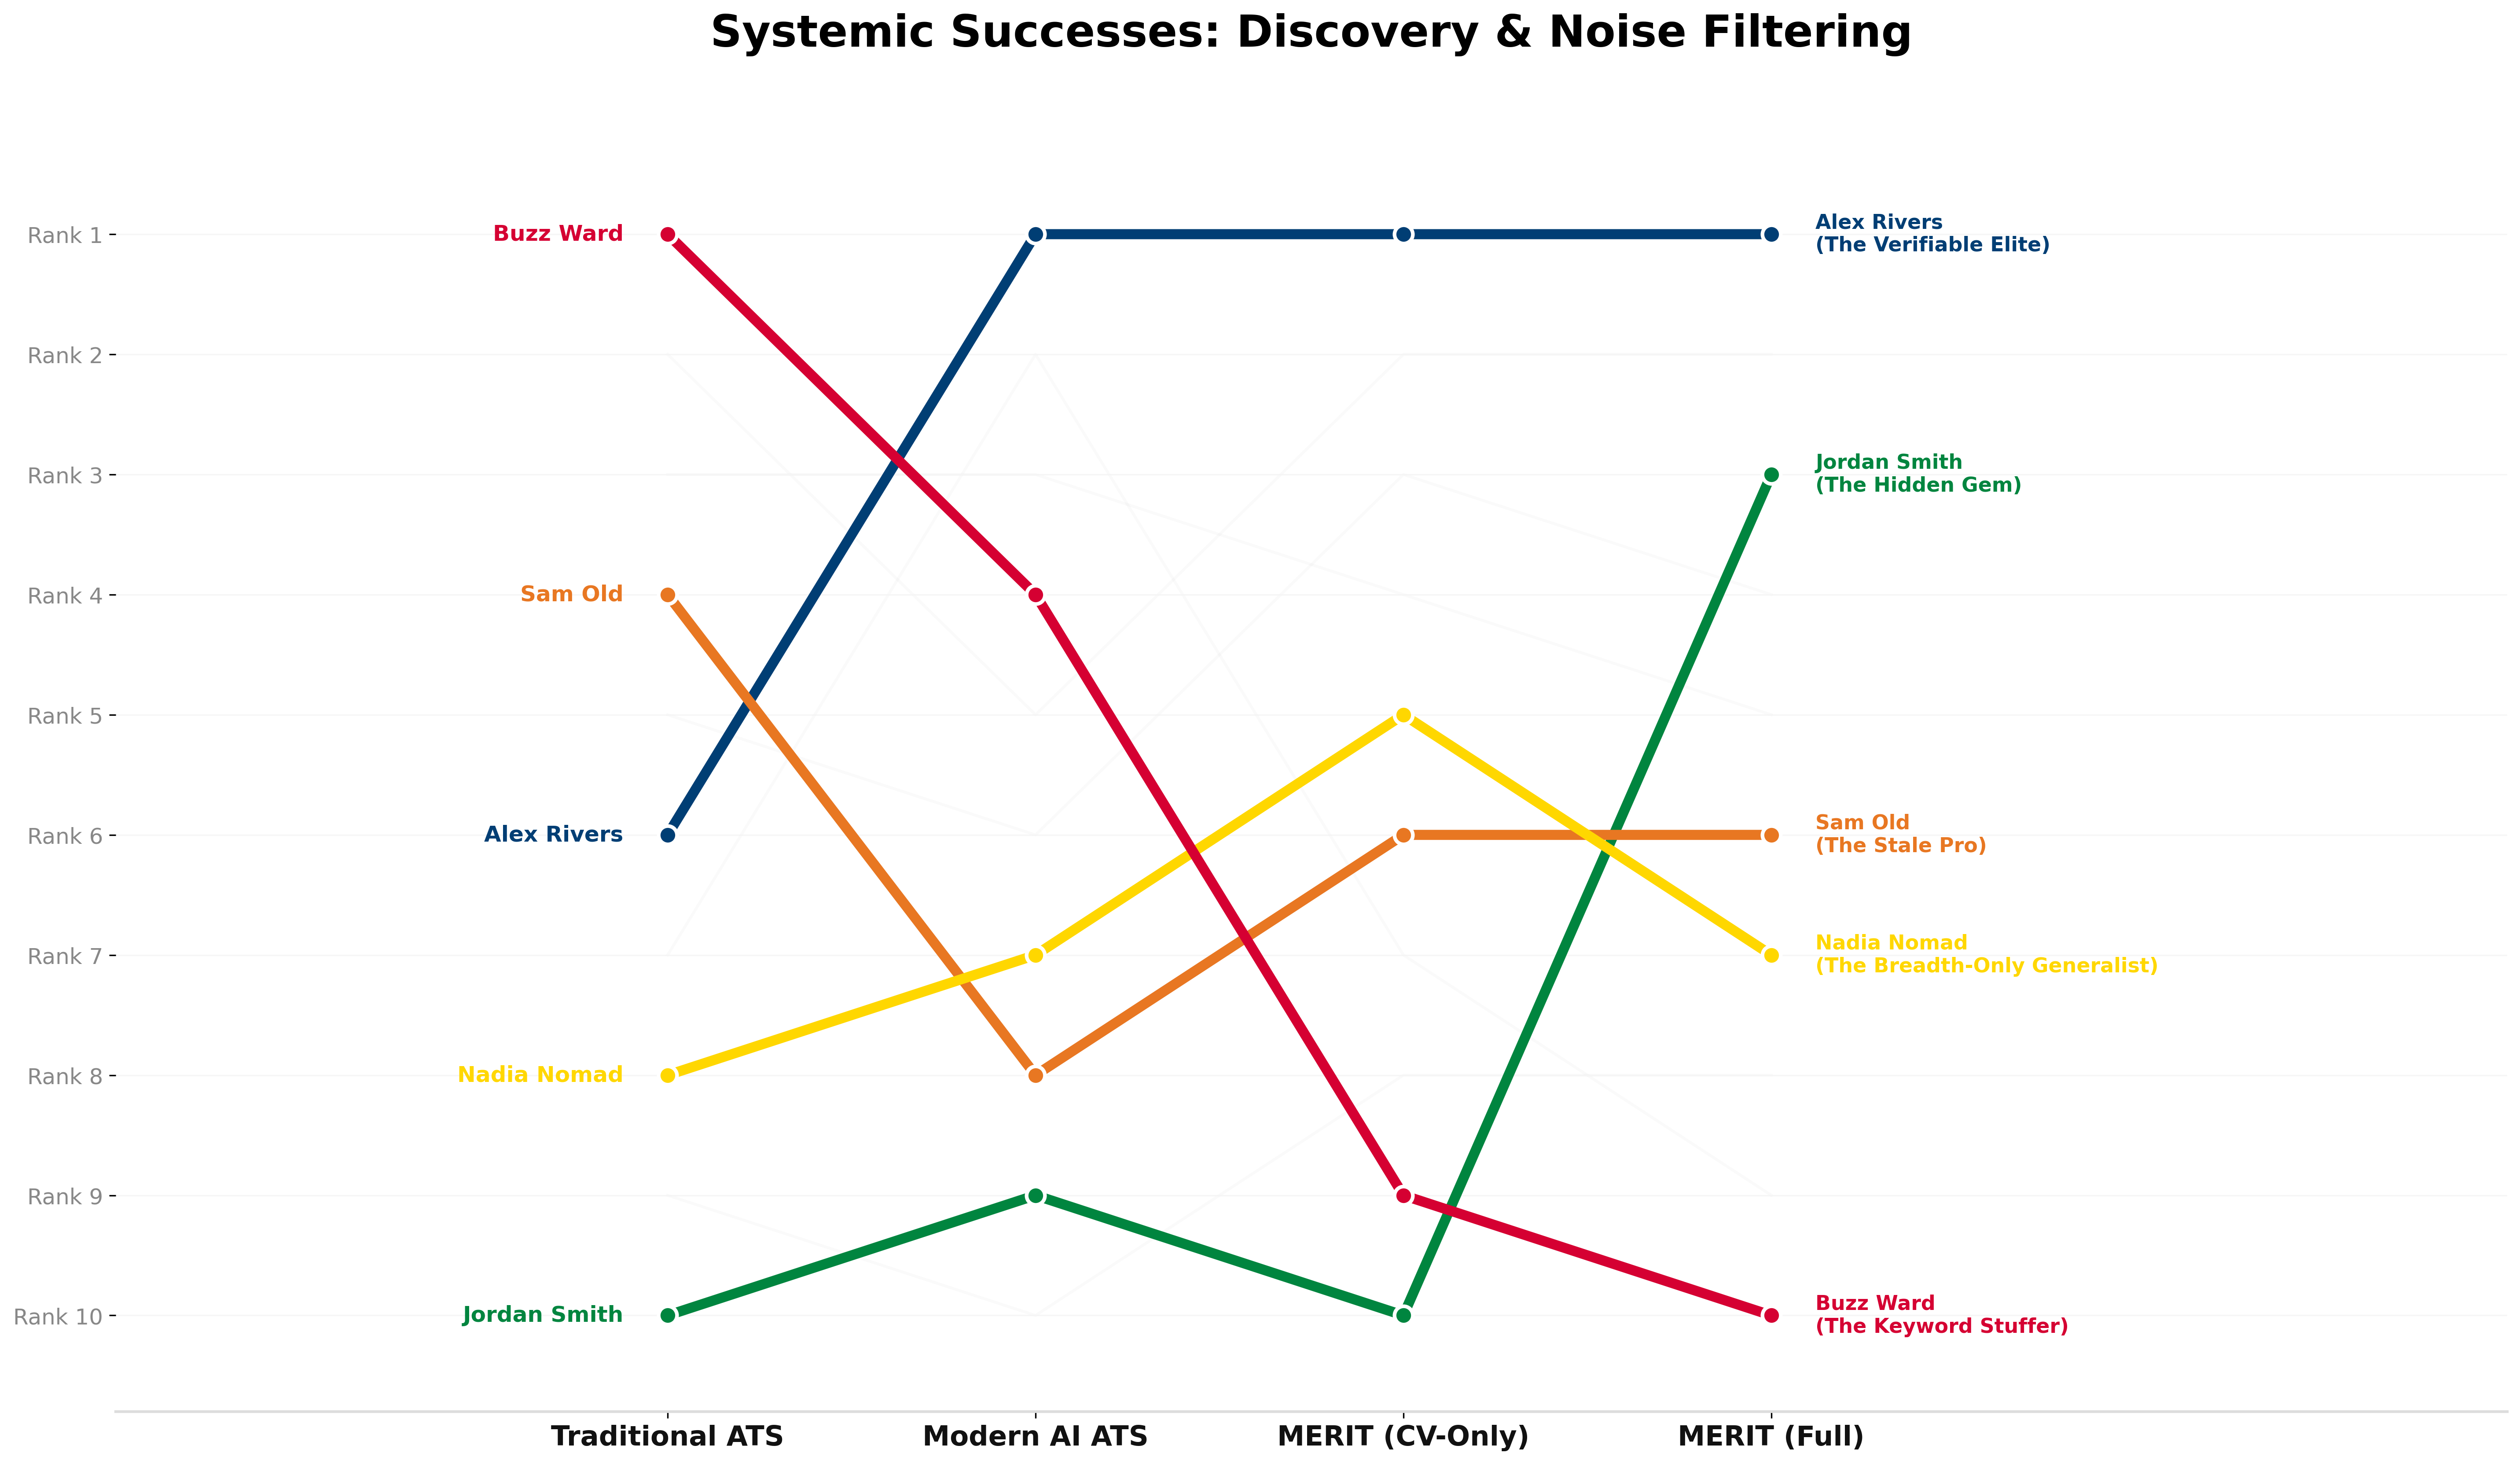
\includegraphics[width=0.95\textwidth]{../evaluation/01-comparative_study/output/rank_displacement_successes.png}
    \caption[Study~01A: Selected rank trajectories]{Study~01A: selected rank trajectories for the key candidates
    of the 10 candidate cohort. We highlight the candidates that are discussed the most in Section~\ref{subsec:study-01a-algorithmic-ablation}
    for better visual clarity. The scores are tabulated in Table~\ref{tab:algorithmic-ablation}.}
    \label{fig:rank-displacement-successes}
\end{figure}

\begin{figure}[htbp]
    \centering
    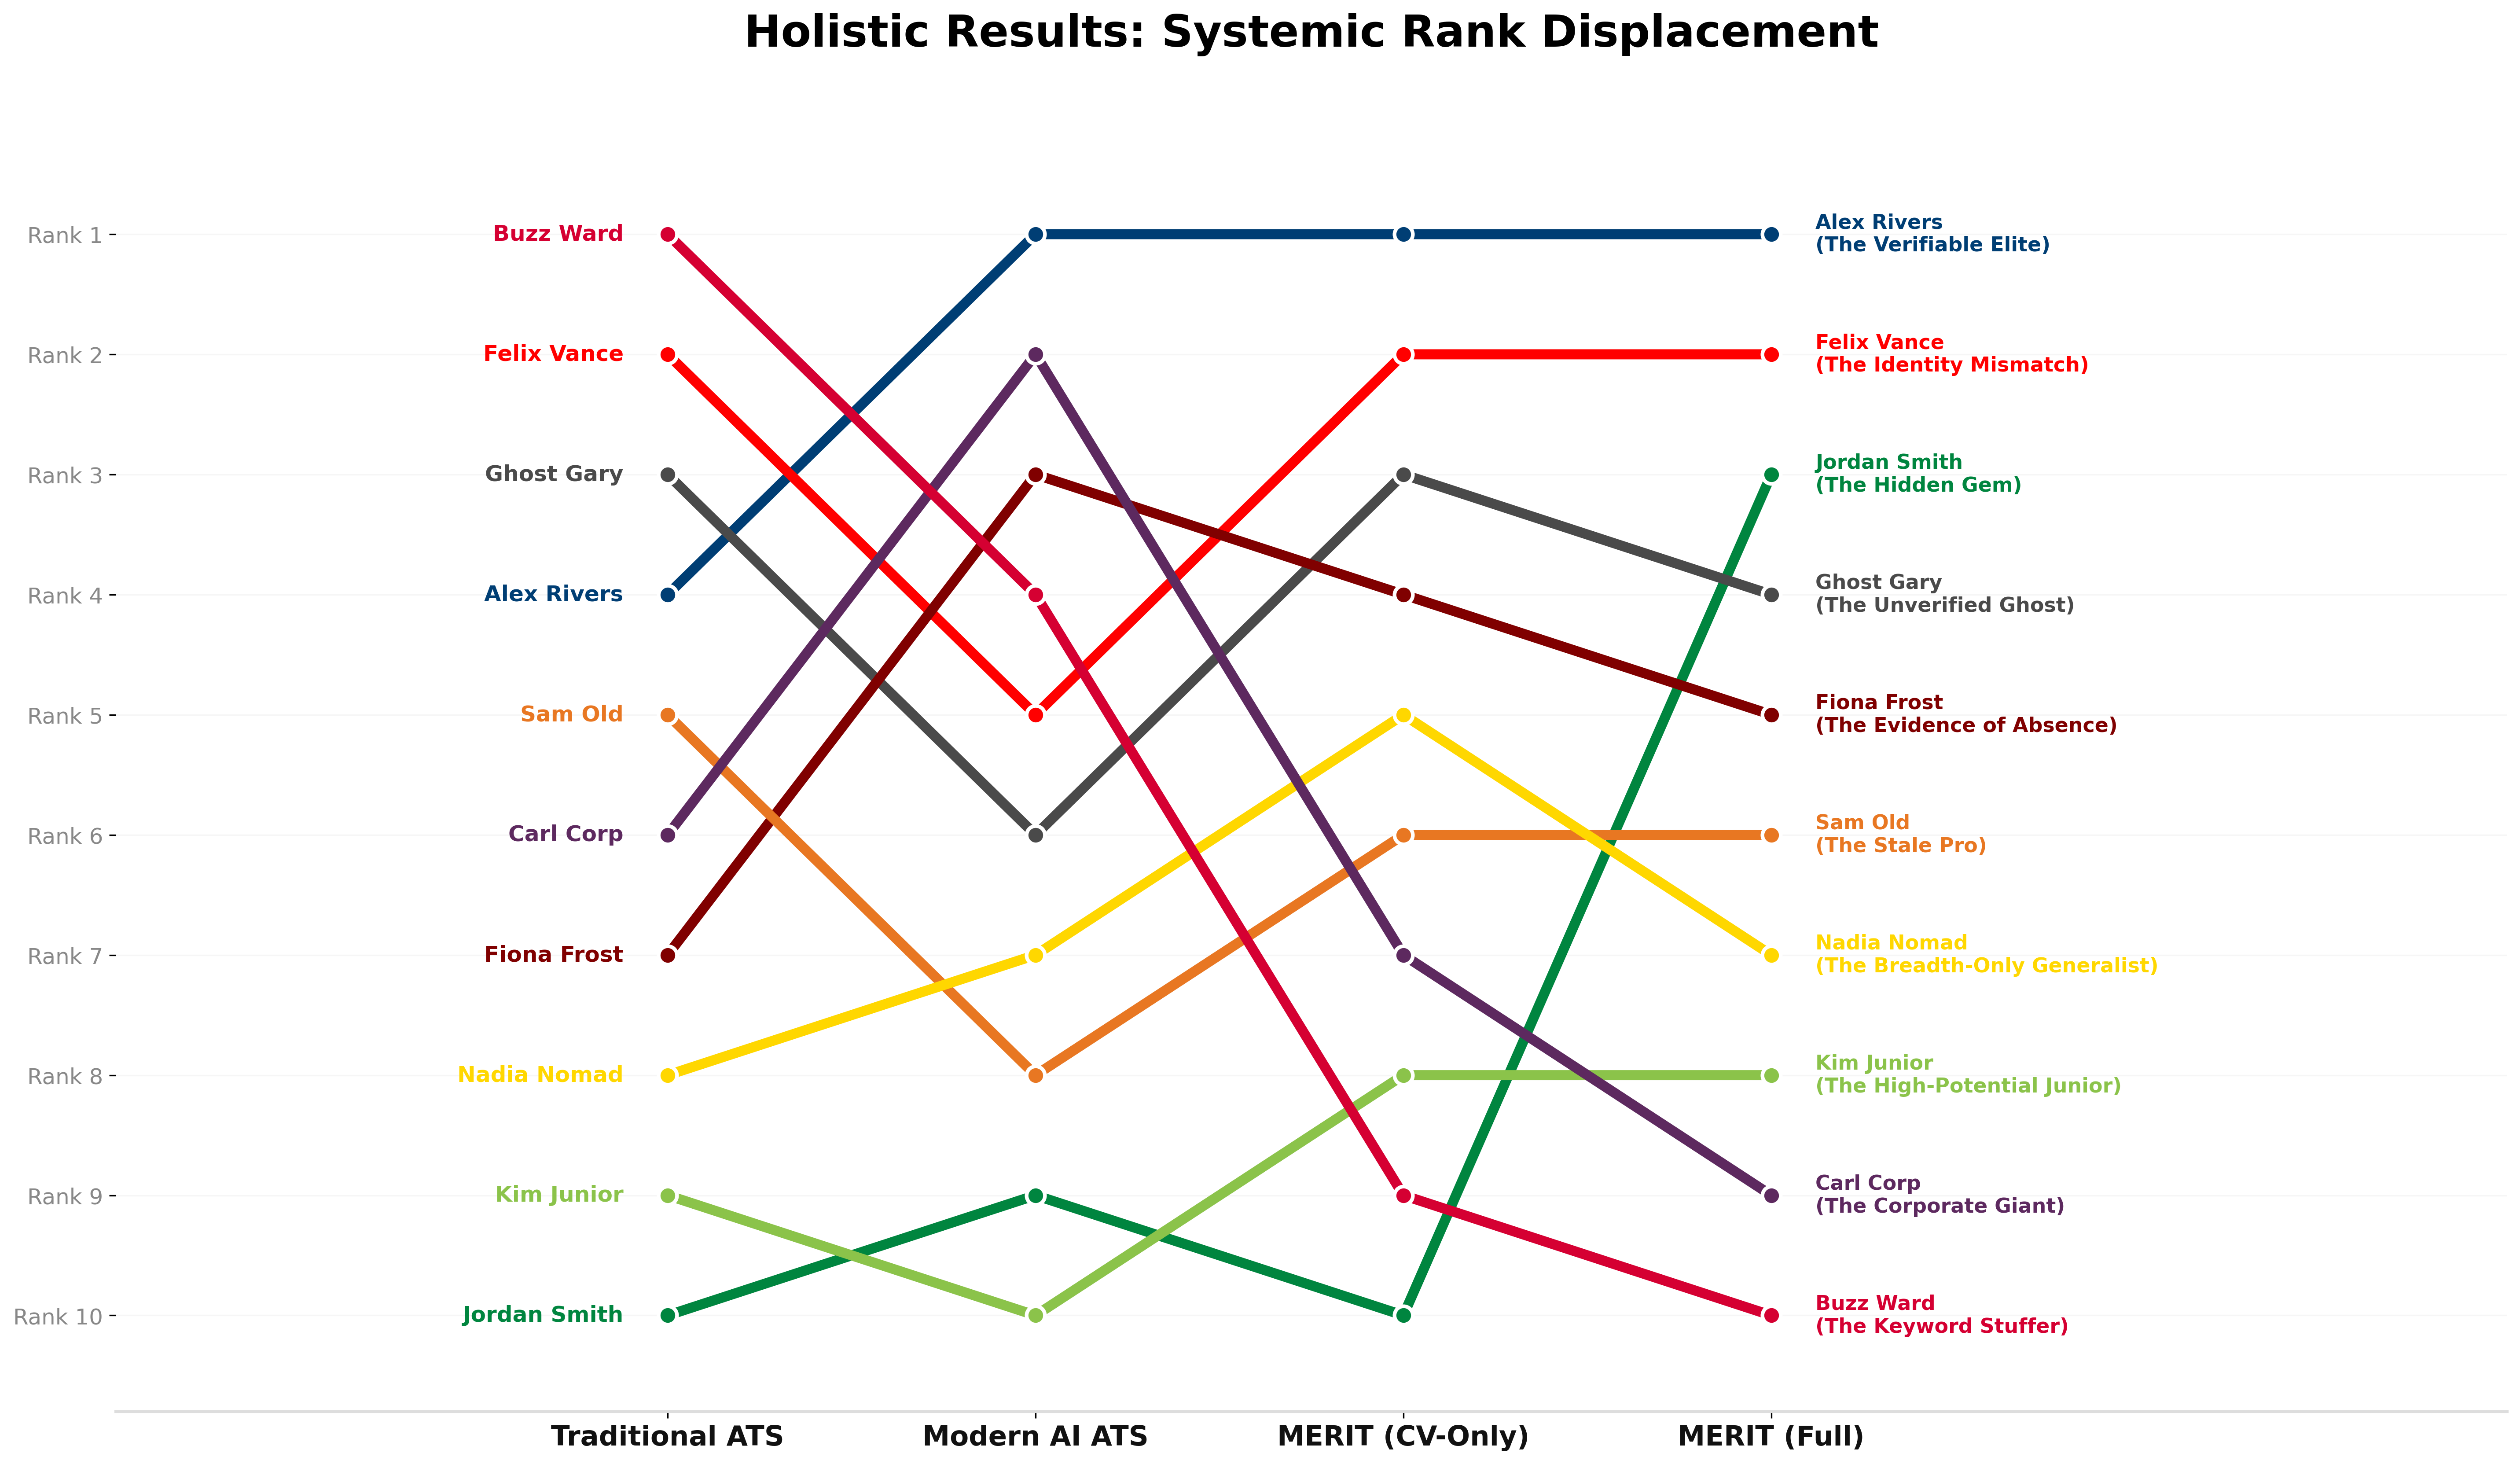
\includegraphics[width=0.92\textwidth]{../evaluation/01-comparative_study/output/rank_displacement_holistic.png}
    \caption[Study~01A: Full rank displacement]{Study~01A: full rank displacement across all ten candidate personas.
    This chart is provided for completeness, refer to Figure~\ref{fig:rank-displacement-successes} 
    for the selected rank trajectories.}
    \label{fig:rank-displacement-holistic}
\end{figure}
